% This is LLNCS.DEM the demonstration file of
% the LaTeX macro package from Springer-Verlag
% for Lecture Notes in Computer Science,
% version 2.4 for LaTeX2e as of 16. April 2010
%
\documentclass{llncs}
%
\usepackage{amsmath}
\usepackage{amssymb}
\usepackage{tikz}

\newcounter{instr}
\newcommand{\ninstr}{\refstepcounter{instr}\theinstr.}

\begin{document}

\title{Species delimitation}

\titlerunning{Species delimitation}

\author{Tom\'{a}\v{s} Flouri1\inst{1} \and Paschalia Kapli\inst{1}}
\authorrunning{Tom\'{a}\v{s} Flouri et al.} % abbreviated author list
\institute{Heidelberg Institute of Theoretical Studies}

\maketitle

\begin{abstract}
An explanation of the GMYC method.
\end{abstract}

\section{Introduction}

We describe the method for delimiting species using the GMYC method presented
in \cite{Fujisawa01092013}.

\section{Preliminaries}

\subsection{Basic definitions}

A tree $T=(V,E)$ is a connected acyclic graph where $V$ is the set of {\em
nodes} and $E$ the set of {\em edges}, such that $E \subseteq V\times V$. We
use the notation $(u,v) \in E$ to denote an edge with end-points $u,v \in V$.
If $T$ is {\em oriented}, then {\em in-degree} (resp. {\em out-degree}) of a
node denotes the number of incoming (resp. outgoing edges) of $u$. In the
opposite case, the {\em degree} of node $u$ denotes the number of edges $u$ is
an end-point of.  Further, we denote with $T_u$ the subtree of $T$ rooted at
node $u$.  A {\em rooted binary tree} $T$ is a {\em directed} tree with all
nodes having in-degree 1 and out-degree 1 ({\em inner} nodes), or in-degree 1
and out-degree 0 ({\em leaves}). Furthermore, one node has in-degree 0 and
out-degree 2 ({\em root}).  In the rest of the text we implicitely assume under
the term tree a binary rooted tree.  We denote the set of leaves of tree $T$ as
$L(T)$.  The cardinality of a set $X$ is denoted as $|X|$. The mapping $\ell :
E \mapsto \mathbb{N}$ associated each edge $e \in E$ with a length $\ell(e)$.
For clarity, we will use the notation $\ell_{u,v}$ to denote the length
$\ell((u,v))$.  We define the {\em height} $h(u)$ of a node $u$ of $T$ as
%
\[ h(u) = \left\{ \begin{array}{ll}
\max(h(v) + \ell_{u,v}, h(w) + \ell_{u,w}) + 1 & \quad : \quad u \notin L(T)\\
0                                                & \quad : \quad u    \in L(T)\\
\end{array}\right. \] 
The height $h(T)$ of a tree $T$ is the height of its root. Finally, we will
implicitely use the notation $r$ for specifying the root of a tree, and
$\ell_{u,v}$ for the length of edge $(u,v)$.  A tree is {\em ultrametric} if
the sum of lengths of edges in the path from a leaf to a root is equal for all
leaves in a tree.

\section{Single-threshold GMYC method}

\paragraph{\bf Interval computation.}
We first compute the possible lines where we can distinguish between a
coalescent and a Yule process. These splits occur always at inner nodes.  Let
$s_1, s_2, \ldots, s_{k+1}$ be the ordered sequence of $k$ values such that
$s_i> s_{i-1}$ for $2 \leq i \leq k+1$ and $\{ h(u) \ |\ \forall u \in V\} = \{
s_1, s_2, \ldots, s_{k+1}\}$.  We obtain $k$ intervals $x_i$ such that $x_i =
s_{i+1} - s_i$ for $1 \leq i \leq k$. Fig.~\ref{fig:tree} shows an example.

\begin{figure}[t]
\centering
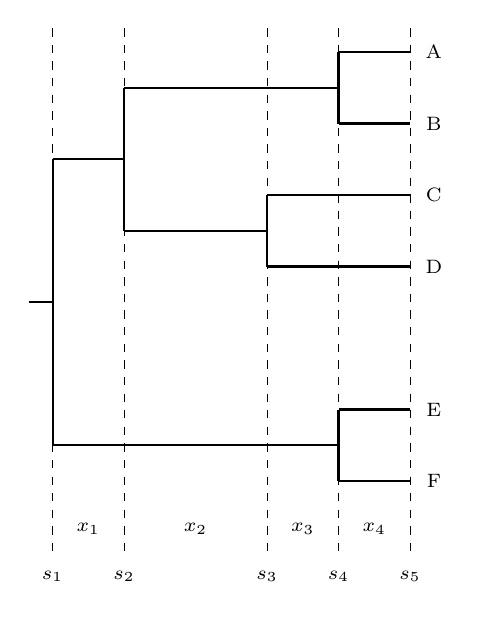
\begin{tikzpicture}[font=\scriptsize]
%\draw[step=1ex,gray,very thin] (0,0) grid (50ex,50ex);
%\draw (0,0ex) -- (40ex,0ex) -- (40ex,50ex) -- (0ex,50ex) -- (0ex,0ex);

\draw [-,thick] (0ex,25ex) -- (2ex,25ex);

\draw [-,thick] (2ex,25ex) -- (2ex,13ex);    % 4xu
\draw [-,thick] (2ex,25ex) -- (2ex,37ex);    % 4xu

\draw [-,thick] (2ex,37ex) -- (8ex,37ex);    % 2xu

\draw [-,thick] (8ex,37ex) -- (8ex,43ex);     % 2xu
\draw [-,thick] (8ex,37ex) -- (8ex,31ex);     % 2xu

\draw [-,thick] (8ex,43ex) -- (26ex,43ex);    %6xu
\draw [-,thick] (26ex,43ex) -- (26ex,46ex);    %1xu
\draw [-,thick] (26ex,43ex) -- (26ex,40ex);    %1xu
\draw [-,thick] (26ex,46ex) -- (32ex,46ex);    %2xu
\draw [-,thick] (26ex,40ex) -- (32ex,40ex);    %2xu


\draw [-,thick] (8ex,31ex) -- (20ex,31ex);    % 4xu
\draw [-,thick] (20ex,31ex) -- (20ex,28ex);    % 1xu
\draw [-,thick] (20ex,31ex) -- (20ex,34ex);    % 1xu
\draw [-,thick] (20ex,34ex) -- (32ex,34ex);    % 4xu
\draw [-,thick] (20ex,28ex) -- (32ex,28ex);    % 4xu

\draw [-,thick] (2ex,13ex) -- (26ex,13ex);    % 8xu
\draw [-,thick] (26ex,13ex) -- (26ex,10ex);    % 1xu
\draw [-,thick] (26ex,13ex) -- (26ex,16ex);    % 1xu
\draw [-,thick] (26ex,16ex) -- (32ex,16ex);    % 2xu
\draw [-,thick] (26ex,10ex) -- (32ex,10ex);    % 2xu

\draw [-, dashed] (2ex,48ex) -- (2ex, 4ex);
\draw [-, dashed] (8ex,48ex) -- (8ex, 4ex);
\draw [-, dashed] (20ex,48ex) -- (20ex, 4ex);
\draw [-, dashed] (26ex,48ex) -- (26ex, 4ex);
\draw [-, dashed] (32ex,48ex) -- (32ex, 4ex);

\node at (2ex,2ex) {$s_1$};
\node at (8ex,2ex) {$s_2$};
\node at (20ex,2ex) {$s_3$};
\node at (26ex,2ex) {$s_4$};
\node at (32ex,2ex) {$s_5$};

\node at (5ex,6ex) {$x_1$};
\node at (14ex,6ex) {$x_2$};
\node at (23ex,6ex) {$x_3$};
\node at (29ex,6ex) {$x_4$};

\node at (34ex,46ex) {A};
\node at (34ex,40ex) {B};
\node at (34ex,34ex) {C};
\node at (34ex,28ex) {D};
\node at (34ex,16ex) {E};
\node at (34ex,10ex) {F};
\end{tikzpicture}

\caption{A tree with four intervals, and 5 inner nodes.}\label{fig:tree}
\end{figure}

\paragraph{\bf Main method.}
Having computed the intervals, the methods proceeds by iteratively setting each
inner node (apart from the root) as the point in time where speciation stops
and coalescence starts, and computes the likelihood of this setting by
optimizing the two values $p_s$ and $p_c$. Once the threshold yielding the
maximum likelihood is found, it is tested against the null hypothesis, and in
case it passes, delimitation is carried based on the threshold, otherwise all
taxa are different species. Fig.~\ref{fig:gmyc-single} illustrates the
single-threshold version of the GMYC algorithm.  The formulas for the
likelihood computation $L$ are for the $k$ intervals are the following.
$$L \leftarrow \sum_{i\leftarrow 1}^k b_i e^{-b_i x_i}$$
where
$$b_i \leftarrow \lambda_s (n_i^s)^{p_s} + \sum_{j\leftarrow 1}^{m_i}\lambda_c(n_{i,j}^c(n_{i,j}^c-1))^{p_c}$$
such that $m_i$ is the number of coalescent events for interval $x_i$. Finally, the rates $\lambda_s$ and $\lambda_c$
are computed as
$$ \lambda_s \leftarrow \frac{i-1}{\sum_{j\leftarrow 1}^k (n_j^s)^{p_s} x_j}$$
considering $s_i$ as the threshold, and
$$ \lambda_c \leftarrow \frac{\sum_{i\leftarrow 1}^k\sum_{j\leftarrow 1}^{m_i}(n_{i,j}^c-1)}{\sum_{i\leftarrow 1}^k\sum_{j\leftarrow 1}^{m_i}(n_{i,j}^c(n_{i,j}^c -1))^{p_c}x_i}.$$
Note that, the nominator for $\lambda_s$ is in fact the number of bifurcations
occuring before the threshold, while the nominator for $\lambda_c$ is the
number of bifurcations occuring after (and including the) threshold.

\setcounter{instr}{0}
\begin{figure}[t]
\begin{center}
\begin{tabular}{|rl|}
\hline
\multicolumn{2}{|l|}{\textsc{DP}$(V, E, k)$}\\
\ninstr & $\textit{max\_L} \leftarrow = -\infty$\\
\ninstr & \textbf{for} $r \leftarrow 2$ \textbf{to} $k+1$\\
\ninstr & \qquad set $s_r$ as threshold\\
\ninstr & \qquad \textbf{for} $i \leftarrow 1$ \textbf{to} $k$\\
\ninstr & \qquad \qquad $m_i \leftarrow $ number of coalescent events at interval $x_i$ \\
\ninstr & \qquad \qquad $n_i^s \leftarrow $ number of speciation lineages at interval $x_i$ \\
\ninstr & \qquad \qquad \textbf{for} $j \leftarrow 1$ \textbf{to} $m_i$\\
\ninstr & \qquad \qquad \qquad $n_{i,j}^c \leftarrow $ number of coalescent lineages in event $j$ of interval $x_i$ \\
\ninstr & \qquad optimize $p_s,p_c$ for minimizing $L$ using L-BFGS-R with $s_r$ as threshold.\\
\ninstr & \qquad $\textit{L} \leftarrow \textsc{Sum-L}(p_s,p_c)$.\\
\ninstr & \qquad \textbf{if} $\textit{L} > \textit{max\_L}$\\
\ninstr & \qquad \qquad $\textit{threshold\_node} \leftarrow u$\\
        & $\rhd$ Run Null Method\\
\ninstr & Optimize $p_s,p_c$ for minimizing $L$ using L-BFGS-R with $s_1$ as threshold.\\
\ninstr & Run likelihood ratio test\\
        & $\rhd$ Delimit species according to $\textit{threshold\_node}$.\\
\hline  
\end{tabular}
\end{center}
\caption{The DP algorithm for computing relative divergence times. The
algorithm starts by passing the tree ($T$), number of discretization lines
(($N$) and the root of $T$ ($u$). It recursively traverses the tree in
postorder and thne computes the best placement for every node $u$.}
\label{fig:gmyc-single}
\end{figure}

\bibliographystyle{splncs03}
\bibliography{delimit}
\end{document}
